\section{Versuchsaufbau und Durchführung}
\label{sec:Versuchsaufbau und Durchführung}
Der Aufbau des Versuches ist in der Abbildung \ref{fig:versuchsaufbau} zu sehen.
\begin{figure}[h]
	\centering
	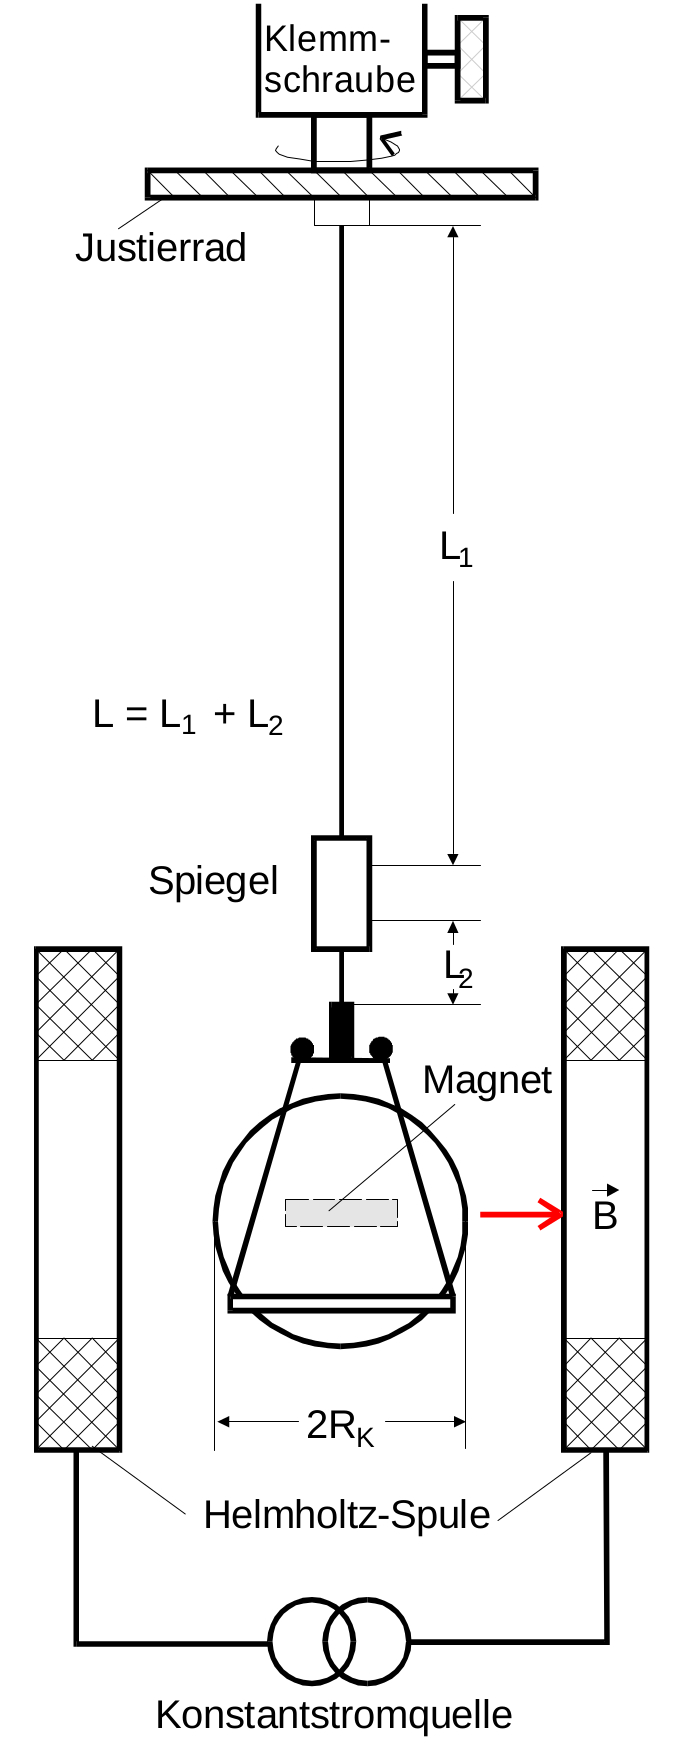
\includegraphics[width=0.7\linewidth]{../../Versuchsaufbau}
	\caption{Foto des Versuchsaufbaus}
	\label{fig:versuchsaufbau}
\end{figure}
Zuerst befindet sich ein Steuergerät auf der linken Seite der Abbildung, wo die entsprechenden Eigenschaften des Magnetfeldes und das Stroboskop eingestellt werden können. Das Luftkissen kann ebenfalls auch an dem Gerät angesteuert werden. Auf der rechten Seite der Abbildung sind die Helmholtz-Spulenpaar mit den Abmessungen $N=195$, $d=\SI{0.138}{\meter}$ und $R=\SI{0.109}{\meter}$ und der Messingzylinder zu sehen. Auf dem Messingzylinder wird eine Billiardkugel gebracht, die sich mit Hilfe des Luftkissens reibungslos bewegen kann und in deren Mitte ein Permanentmagnet vorhanden ist. 
\subsection{Statische Methode unter Verwendung der Gravitation}
Für den ersten Typ der experimentellen Bestimmung des magnetischen Momentes wurde zuerst eine verschiebbare Masse $m$  an der Aluminiumstange in der Billiardkugel angefügt. Dazu wird das Luftkissen eingeschaltet sodass die Feldrichtung nach oben zeigte. Hierbei musste die Masse so oft verschoben und der Strom so festgelegt werden, bis sich das System in einem Gleichgewicht befand. Dabei wurde der Radius $r$ der kleinen Masse $m$ vom Zentrum der Billiardkugel für mindestens $10$ Messungen festgelegt. Zudem wurde die Masse des Aluminiumstifts für die Berechnung ignoriert und die kleine verschiebbare Masse als Punktmasse angesehen. 
\subsection{Dynamische Methode unter Verwendung der Schwingungsdauer}
Für den zweiten Typ wurde das Magnetfeld eingeschaltet und die Billiardkugel auf dem Messingzylinder gestellt. Dabei wurde die Billiardkugel so ausgelenkt, dass sie Schwingungen ausführen kann wie bei einem harmonischen Ozillator und die Stromstärke für mindestens $9$ Messungen festgelegt. Die Schwingungsdauer $T$ und die Stromstärke $I$ wurden ebenfalls für mindestens $9$ Messungen aufgeschrieben.
\subsection{Dynamische Methode unter Verwendung der Präzession}
Für den letzten Typ der experimentellen Betrachtung wurde die Billiardkugel auf das Luftkissen gesetzt, das Luftkissen eingeschaltet, und das Stroboskop auf eine Frequenz von mindestens $\SI{4}{\Hz}$ gestellt. Als nächstes wurde die Kugel in Rotation versetzt und entsprechend gewartet, bis der weiße Punkt auf dem Stiel stationär war. Zu sehen war auch das Stroboskoplicht, das ständig Lichtblitze gesendet hat, für die Betrachtung des weißen Punktes auf der Kugel. Danach wurde die Kugel mit einem Stift in Auslenkung gebracht und die Spulenstromstärke bei einer geeigneten Frequenz eingeschaltet. Für eine Magnetfeldstärke wurden drei verschiedene Schwingungsdauer gemessen und die gemessenen Daten notiert. Insgesamt wurde die Messung mindestens $10$ mal durchgeführt.
